\section{Timeline}

The following section describes the project development, progress and decision as we did through the time the the project was developed. After series of informal talk the project officially started in December 2011 and was submitted in September 2012.

\subsection{Initial project meetings and early implementation decisions}

The regular project meeting where we discussed mostly the organizational aspects and the top-level design of the application started in December 2011. We easily agreed that we were aiming to create an application quite similar to the Google Documents. We have decided very early to use the multi tier architecture consisting of

\begin{itemize}
\item core translation memory,
\item userspace,
\item graphical user interface,
\end{itemize}

who became separate Maven modules. Although we added further modules later, we consistently kept the initial project separation into \emph{Core}, \emph{Userspace} and \emph{GUI}. At the beginning we also assigned team members to the different part of project which remained surprisingly stable as well. 

Before receiving the data from OpenSubtitles.org we were also thinking about the source of data to fill the translation memory for the first time. There were several option -- either using the subtitle part of the Czech-English parallel corpus CzEng developed at ÚFAL, using sentences from a general purpose parallel corpus or getting the data from a subtitle server.

Another issue we widely discussed at the beginning was choosing the database system. The database beneath the Translation Memory plays a crucial role for the whole system performance. Also using built-in features could save us a lot of additional work.



\begin{itemize}
	\item We decided to base the project on the \emph{Java Virtual Machine}. Most parts should be written in Java and some parts would be written in the Scala programming language.
	\item For dependency management, we decided to use Apache Maven.
\end{itemize}

\noindent\textbf{Discussion of the decisions}

\begin{itemize}
	\item We are generally satisfied with the decision to base the project on the JVM since both the usage of Google Web Toolkit and other modules, as well as the possibility to combine all parts of the project with Apache Maven were helpful. 
	
	The decision to use both Java and Scala showed to be a difficult decision. On the one hand, Scala allowed to write concise and efficient code, on the other hand most project members were not able to learn Scala sufficiently and hence used only Java. Although the interoperability between Scala and Java works well in most cases because both are based on the JVM, some problems remain. One of the problems of interoperability was, for example, that the implementation of the datatype \emph{List} that was created in Scala was not compatible with Google Web Toolkit, which expected a standard Java \emph{List} implementation.
\end{itemize}


\begin{itemize}
	\item  Initially, the scripts for preparing the initial data were written in Perl and classes to import the data were in the \emph{Core} module. However, to be more consistent, we decided to move the data preparation and data import to a separate \emph{dataimport} module and re-wrote the Perl scripts in Scala.
\end{itemize}

\begin{figure}[h]
\begin{center}
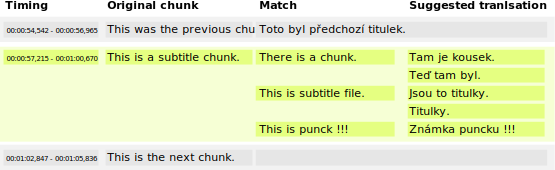
\includegraphics{./figures/original_strucutre.pdf}
\end{center}

\caption{Scheme of the originally intended structure of work with the translation memory. It reflects the original User Space structure and also schematically the original client design.}

\end{figure}

\subsection{Database evaluations and choice of GUI framework}

\begin{itemize}
	\item We evaluated different DBMS and decided to use Postgres (see section~\ref{sec:dbms}).
	\item We decided to use Google Web Toolkit for the GUI.

\end{itemize}


\subsection{Agreement on shared classes}

\begin{itemize}
	\item We agreed on the shared classes that all parts of the project should use. For best compatibility between  \emph{Core}, \emph{Userspace} and the GWT-based \emph{GUI}, we decided to write all shared classes in Java.
\end{itemize}


\noindent\textbf{Discussion of the decision}

\begin{itemize}
	\item It showed to be an important decision to agree on the shared classes early in the project since it made the cooperation between the modules easier and less verbose.
\end{itemize}


\subsection{Core design decisions}



\subsection{User Space design decisions}



\subsection{GUI design decisions}

\section{Evaluating the Development Process}

One of the crucial decision for the project was the choice of technologies. Most of the technologies we used -- Maven, Scala, Hibernate, GWT -- were new to all of us and we also had not much experience with the other. Combining these technologies together was quite painful and would probably even for an experienced Java developer. Generally, we can say that the fact that we were not too much familiar with the technologies, we spent most of the time solving technical issues. There is quite a lot of research challenges, mostly in the fuzzy matching part, which had to remain untouched due to that.

On the other hand the choice of technologies appeared to be lucky that it probably saved a lot of work for us by the possibility to share implementation of class. Using the Scala language for the core also made the parallelization much easier.

Despite we spent quite a lot of time by the discussions how the structure of the project we didn't avoid a radical change of the design of the application 4 months after the project started. Nearly the whole User Space code had to be dropped and it was also necessary to totally remake the client components existing so far.





